% Encoding: utf-8
% Format: LaTeX-Beamer
% Lukas Pospisil, Petr Kovar
% Last update: 29.01.2012
%%%%%%%%%%%%%%%%%%%%%%%%%%%%%%%%%%%%%%%%%%%%%%%%%%%%%%%%%%%%%%%%%%%%%%

\documentclass{beamer}
\usepackage{amsmath}
% Packages to use
%\usepackage[cp1250]{inputenc} % Windows
\usepackage[utf8]{inputenc} % Unix/Linux
\usepackage[czech]{babel}
%\usepackage[english]{babel}
\usepackage{graphicx}
\usepackage{color}

\usepackage{graphicx}
\usepackage{float} 
\usepackage{pgfplots} 
\usepackage{listings}
\usepackage{xspace}

% Use the KAM theme in beamerthemeKAM.sty
\usetheme{KAMcz}
%\usetheme{KAMen}

%%%%%%%%%%%%%%%%%%%%%%%%%%%%%%%%%%%%%%%%%%%%%%%%%%%%%%%%%%%%%%%%%%%%%%
% Makra


%%%%%%%%%%%%%%%%%%%%%%%%%%%%%%%%%%%%%%%%%%%%%%%%%%%%%%%%%%%%%%%%%%%%%%
% Titlepage

\author{Martin Koběrský} % author
\title{Po částech lineární regrese} % name of the presentation
\date{\today} % date
\institute{Katedra aplikované matematiky, VŠB -- TU Ostrava} % instituce CZ


% the ``Thank you'' page
\def\makethanks{%
	\begin{frame}
	\frametitle{\@thankstitle}
	\@thanksmessage
\end{frame}
}
% in ``article'' mode there's no ``Thank you'' page
\mode<article>
{\providecommand\makethanks{}}

% commands for the title and message of the "Thank you" page
\def\thankstitle#1{\def\@thankstitle{#1}}
\def\thanksmessage#1{\def\@thanksmessage{#1}}

\thankstitle{Děkuji za pozornost!}
\thanksmessage{}

%%%%%%%%%%%%%%%%%%%%%%%%%%%%%%%%%%%%%%%%%%%%%%%%%%%%%%%%%%%%%%%%%%%%%%
% Presentation begins
%%%%%%%%%%%%%%%%%%%%%%%%%%%%%%%%%%%%%%%%%%%%%%%%%%%%%%%%%%%%%%%%%%%%%%

\begin{document}

%%%%%%%%%%%%%%%%%%%%%%%%%%%%%%
% Title frame
\begin{frame}
\titlepage
\end{frame}

\begin{frame}
\frametitle{Model}
\begin{figure}
	[H]\centering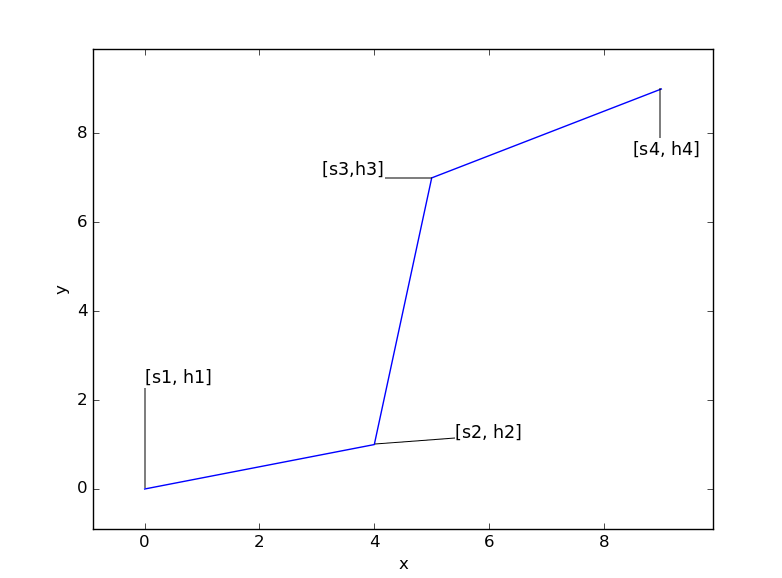
\includegraphics[width=0.8\textwidth]{images/model2.png}
\end{figure}
\end{frame}

%%%%%%%%%%%%%%%%%%%%%%%%%%%%%%
\begin{frame}
\frametitle{Množina parametrů}
  \begin{align*}
	  \theta_2 = (\sigma^2, s_1, h_1, s_2, h_2, s_3, h_3, s_4, h_4)
  \end{align*}
  \begin{align*}
  	   \theta_k = (\sigma^2, s_1, h_1, ..., s_{k+2}, h_{k+2})
  \end{align*}
  \begin{align*}
  		\theta = \bigcup_{k \in K}  \{ k \} \times \theta_k
  \end{align*}
\end{frame}

\begin{frame}
\frametitle{Apriorní rozdělení}
\begin{align*}
    f(\theta) = f(k)f(\theta_1)...f(\theta_K)
\end{align*}
\begin{itemize}
	\item $f$ jsou různé funkce, které rozlišujeme argumentem
	\item každé $f$ používá jinou míru
	\item apriorním rozdělením zaručujeme správné pořadí
\end{itemize}
\end{frame}

\begin{frame}
\frametitle{Aposteriorní rozdělení}
	\begin{align*}
		f(k, \theta_0, \theta_1, ..., \theta_K | y) 
	\end{align*}
	\begin{itemize}
		\item Pravděpodobnostní rozdělení na modelu $f(k | y)$
		\item Pravděpodobnostní rozdělení na konkrétním parametru  $f(\theta_k | y)$
	\end{itemize}
\end{frame}

\begin{frame}
\frametitle{MCMC}
	\begin{itemize}
		\item Markov Chain Monte Carlo
		\item algoritmus konstruující markovovský řetězec
		\item stacionární distribucí je aposteriorní rozdělení
		\item neumožňuje přeskoky mezi dimenzemi
	\end{itemize}
\end{frame}
\begin{frame}
\frametitle{RJMCMC}
	\begin{itemize}
		\item Reversible Jump Markov Chain Monte Carlo
		\item umožňuje přeskoky mezi dimenzemi
		\item dimenze se dorovnává náhodnými veličinami
	\end{itemize}
\end{frame}

\begin{frame}
\frametitle{Numerické experimenty}
\begin{figure}
	[H]\centering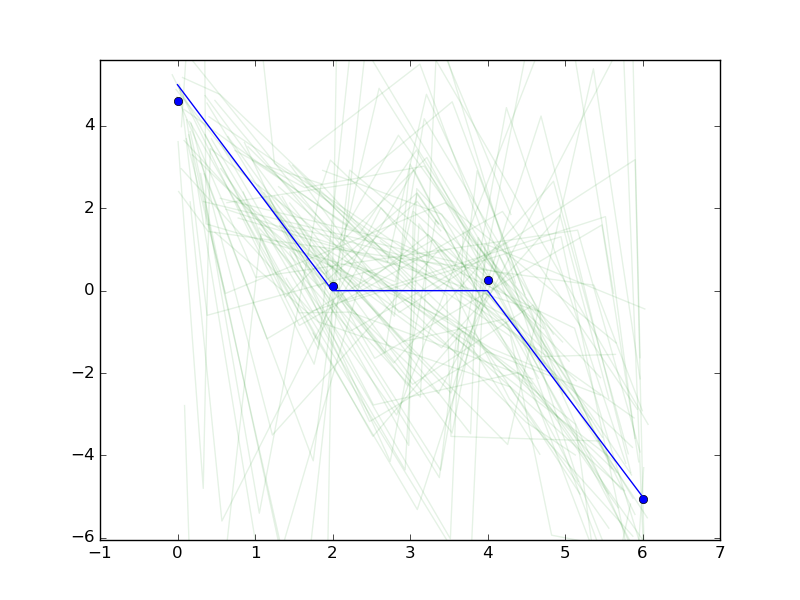
\includegraphics[width=0.8\textwidth]{images/prezentace1_lines.png}
\end{figure}
\end{frame}
\begin{frame}
\frametitle{Numerické experimenty}
\begin{figure}
	[H]\centering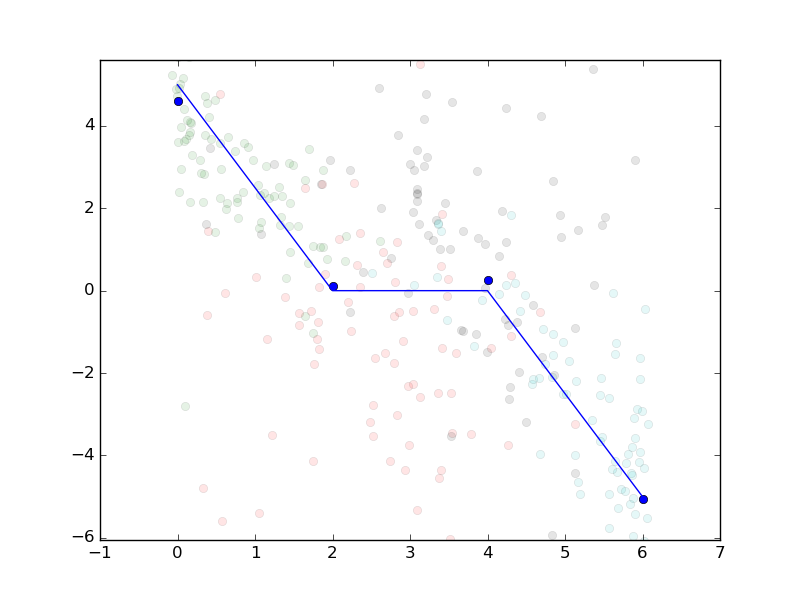
\includegraphics[width=0.8\textwidth]{images/prezentace1_hists.png}
\end{figure}
\end{frame}
\begin{frame}
\frametitle{Numerické experimenty}
\begin{figure}
	[H]\centering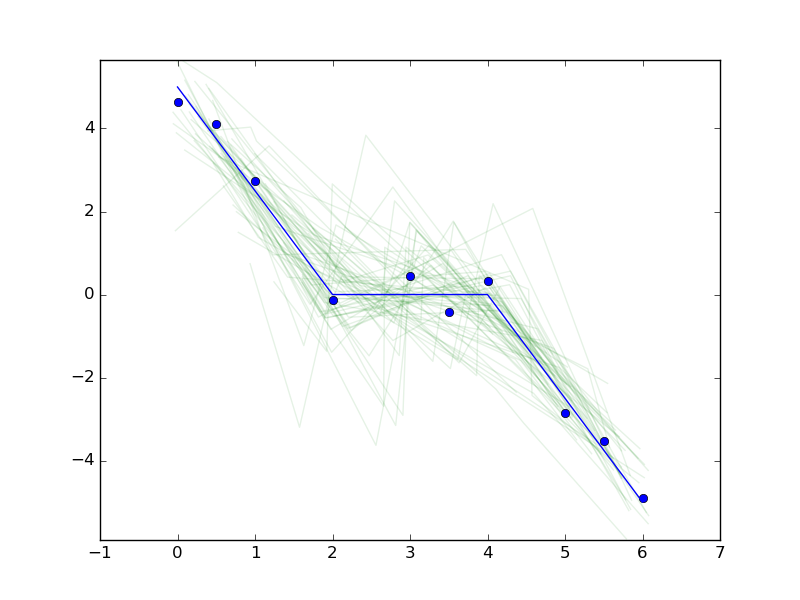
\includegraphics[width=0.8\textwidth]{images/prezentace2_lines.png}
\end{figure}
\end{frame}
\begin{frame}
\frametitle{Numerické experimenty}
\begin{figure}
	[H]\centering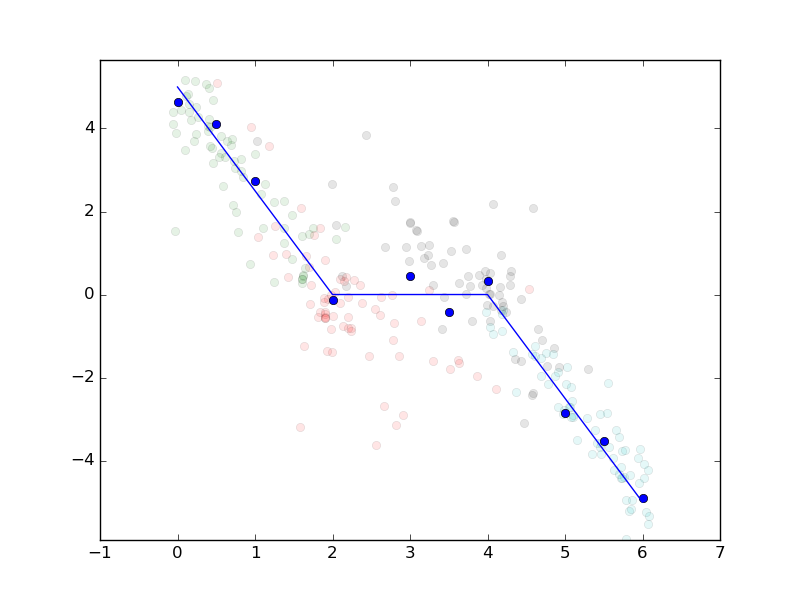
\includegraphics[width=0.8\textwidth]{images/prezentace2_hists.png}
\end{figure}
\end{frame}

\begin{frame}
Děkuji za pozornost.
\end{frame}

\end{document}

%%%%%%%%%%%%%%%%%%%%%%%%%%%%%%%%%%%%%%%%%%%%%%%%%%%%%%%%%%%%%%%%%%%%%%
% end of file "prezentace_kam_cz_utf8.tex"
